\FloatBarrier
\subsection{Question 3}
Since we are not cancelling the zeros of the system $degA_o = degA-degB-1=0$ so we implement  $A_o =  [1]$ as a constant.
\autoref{code:str31} and \autoref{code:str32} show the required steps to calculate the proper control output. The values of $R$ , $S$ and $T$ are directly estimated using RLS . \autoref{fig:str31} shows the system output and control effort for direct STR without zero cancellation.  \autoref{fig:str32} demonstrates the variation of parameter values over simulation time.

\begin{code}
	\begin{matlabcode}{firstnumber = 1}
	cancel = 0; % 0 no zero cancel, 1 all zero cancel
	%% generate Data
	uc = u1 ;
	lamda = 1;
	system_dig = Gz; %system
	[B  ,A] = tfdata(system_dig) ;
	A = cell2mat(A) ;
	B = cell2mat(B) ; B = B(2:end) ;
	% reference model
	Am = [1 -1.7 0.92 -0.16];
	if cancel
		sys_ref_dig = tf([0 sum(Am) 0],Am,Gz.Ts) ;
		A0 = [roots(B)'];
	else
		beta = sum(Am)/sum(B);
		sys_ref_dig = tf(beta*B,Am,Gz.Ts) ;
		A0 = [1];
	end
	[Bm  ,Am] = tfdata(sys_ref_dig);
	Am = cell2mat(Am) ;
	Bm = cell2mat(Bm) ; Bm = Bm(2:end) ;
	y_ref = lsim(sys_ref_dig , uc , t) ;
	%% initial parameters
	n = numel(A)-1 ;
	m = numel(B)-1 ;
	d0 = n-m ;
	A0Am = conv(A0 , Am) ;
	Na0am = numel(A0Am)-1 ;
	L = Na0am-d0 ;
	Nv = 3*(L+1) ;
	teta = zeros(Nv , 1) ;
	P = 1e4*eye(Nv) ;
	u  = randn(Nv , 1) ;  % initial effort control
	y  = randn(Nv , 1) ;  % initial output
	uf = randn(Nv , 1) ;  % initial filtered effort control
	yf = randn(Nv , 1) ;  % initial filtered output
	ucf= randn(Nv , 1) ;  % initial filtered command signal
	N = numel(t) ;
	for i =1:Nv
		tetas(:,i) = teta;
	end
		\end{matlabcode}
	\captionof{listing}{Parameters of direct STR without zero cancellation}
	\label{code:str31}
\end{code}
	\begin{code}
		\begin{matlabcode}{firstnumber = 1}
	%% main loop
	for i = Nv+1:N
		y(i) = -A(2:end)*y(i-1:-1:i-n)+B*(u(i-d0:-1:i-n)) ;
		U = uf(i-d0:-1:i-L-d0) ;
		V = [yf(i-d0:-1:i-L-d0)' , -ucf(i-d0:-1:i-L-d0)']' ;
		Y = y(i)-y_ref(i) ;
		
		[teta , P] = RLS(U , V , Y , teta , P , Nv,lamda) ;
		tetas(:,i)=teta;
		
		Rst = teta(1:Nv/3)' ;
		Sst = teta(Nv/3+1:2*Nv/3)' ;
		Tst = teta(2*Nv/3+1:Nv)' ;
		
		u(i) = (-Rst(2:end)*u(i-1:-1:i-L)+Tst*uc(i:-1:i-L)-Sst*y(i:-1:i-L))/Rst(1) ;
		uf(i) = -A0Am(2:end)*uf(i-1:-1:i-Na0am)+u(i) ;
		yf(i) = -A0Am(2:end)*yf(i-1:-1:i-Na0am)+y(i) ;
		ucf(i) = -A0Am(2:end)*ucf(i-1:-1:i-Na0am)+uc(i) ;
	end
	\end{matlabcode}
	\captionof{listing}{Basic impelementation of direct STR}
	\label{code:str32}
\end{code}

\begin{figure}
	\centering
	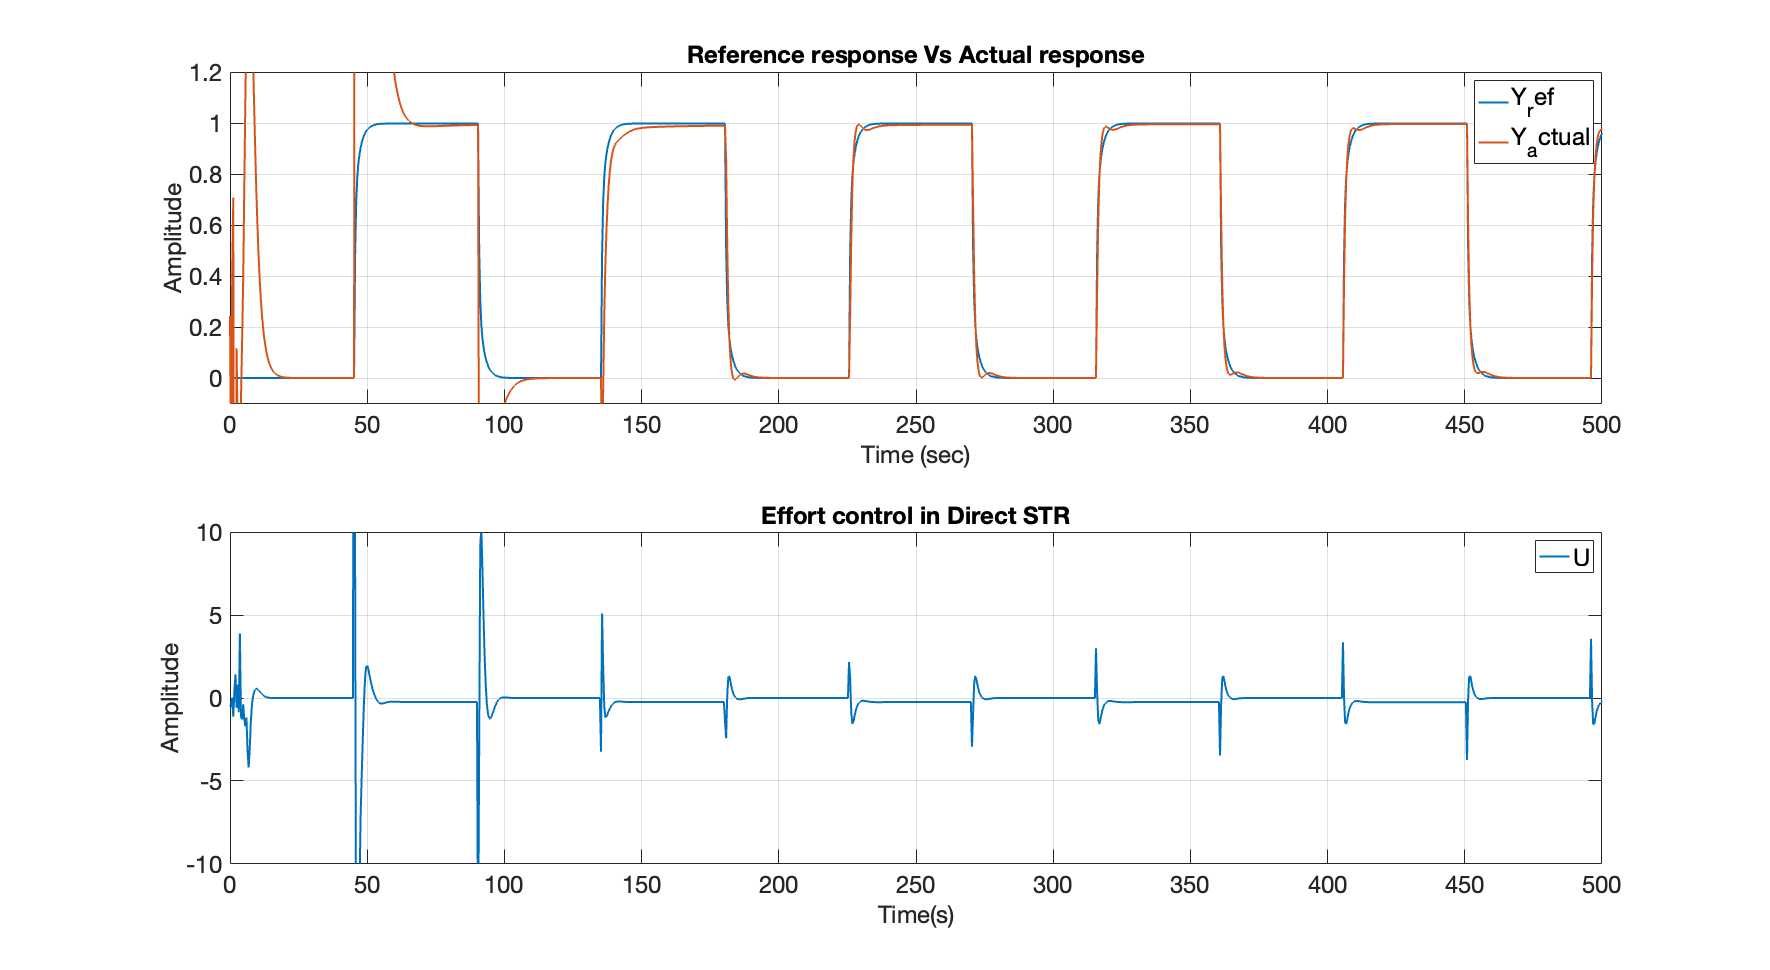
\includegraphics[width=\textwidth]{images/str31.png}
	\caption{System response without zero cancelling direct STR }
	\label{fig:str31}
\end{figure}

\begin{figure}
	\centering
	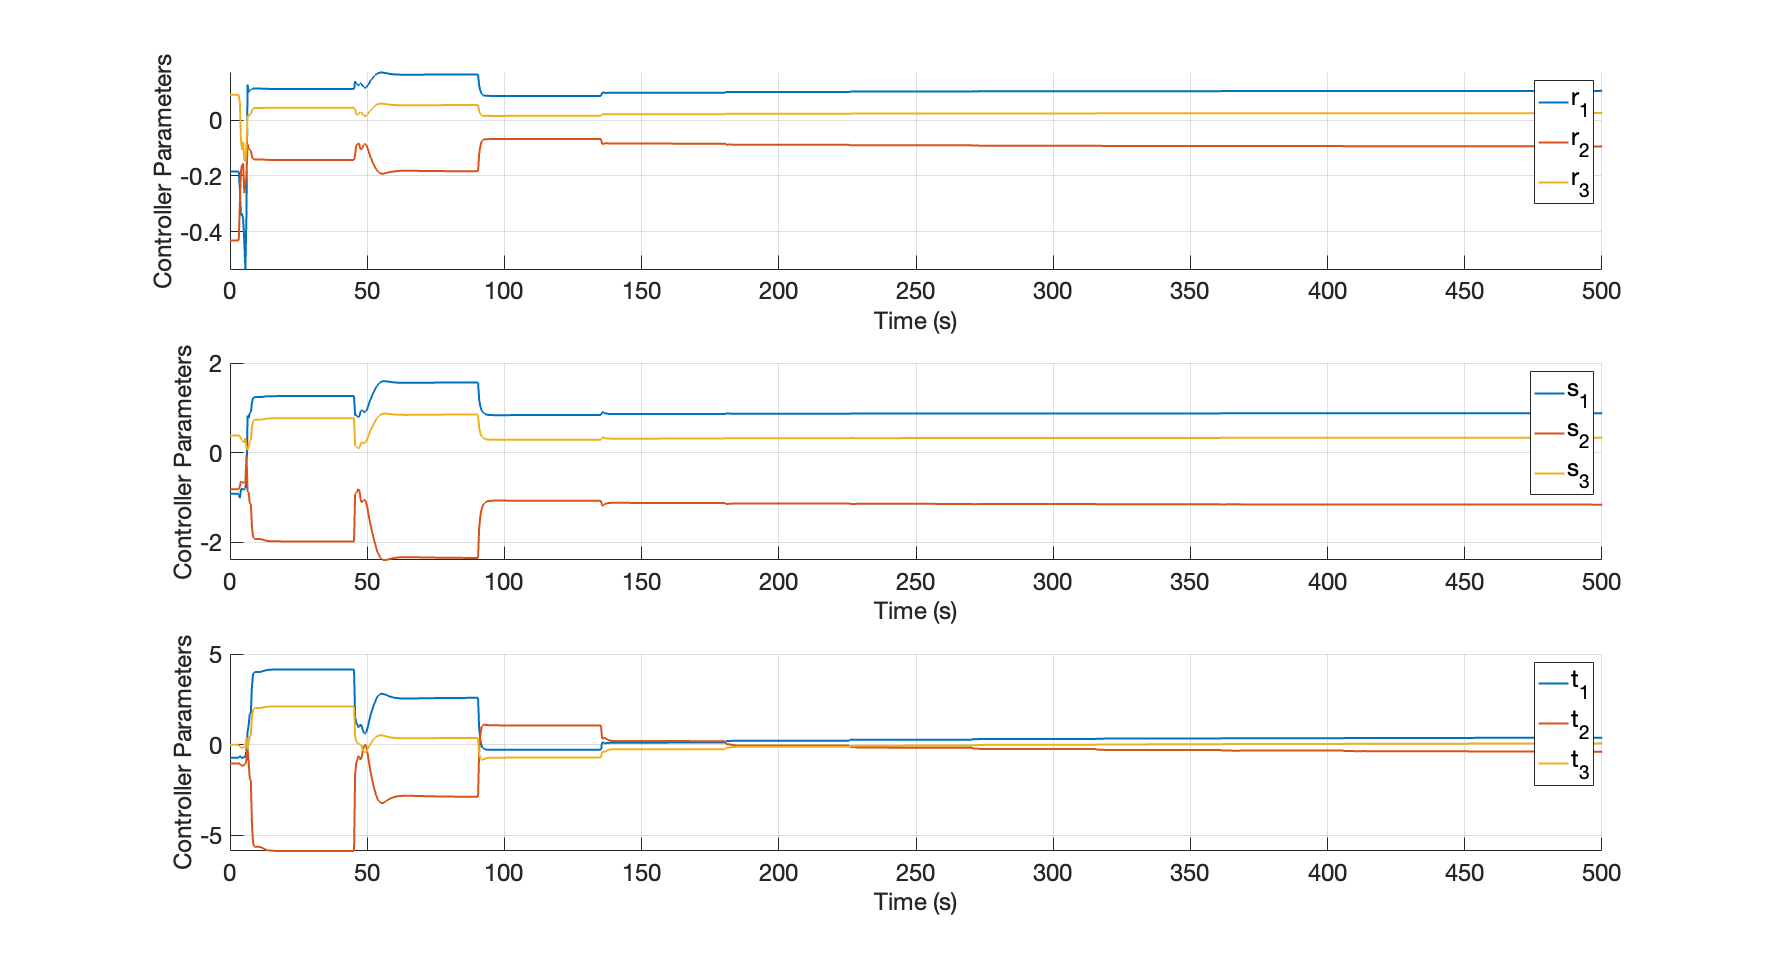
\includegraphics[width=\textwidth]{images/str32.png}
	\caption{System parameters in direct STR without zero cancellation}
	\label{fig:str32}
\end{figure}

The code  for this section is available at \lstinline|assignment2/part2/STR1_direct.m|. RLS impelementation is located at \lstinline|assignment2/part2/RLS.m|.
